\chapter{Chapter 1}
\label{sec:ap1}

\clearpage

\section{Vindex Tables}
\label{sec:vin_tables}

\begin{table}[!ht]
    \centering
\begin{tabular}{lcc}
	\hline
	Category & Vindex & SE \\
	\hline \hline
cigarettes       & 0.76 & (0.014) \\
cars             & 0.72 & (0.012) \\
clothing         & 0.70 & (0.013) \\
furniture        & 0.68 & (0.012) \\
jewelry          & 0.67 & (0.015) \\
recreation 1     & 0.66 & (0.012) \\
food out         & 0.61 & (0.012) \\
alcohol home     & 0.60 & (0.014) \\
barbers etc      & 0.60 & (0.014) \\
alcohol out      & 0.59 & (0.014) \\
recreation 2     & 0.57 & (0.013) \\
books etc        & 0.57 & (0.013) \\
education        & 0.56 & (0.014) \\
food home        & 0.51 & (0.014) \\
rent/home        & 0.49 & (0.016) \\
cell phone       & 0.46 & (0.016) \\
air travel       & 0.46 & (0.014) \\
hotels etc       & 0.45 & (0.013) \\
public trans     & 0.44 & (0.015) \\
car repair       & 0.42 & (0.014) \\
gasoline         & 0.39 & (0.016) \\
health care      & 0.36 & (0.014) \\
charities        & 0.34 & (0.014) \\
laundry          & 0.33 & (0.015) \\
home utilities   & 0.31 & (0.015) \\
home phone       & 0.29 & (0.015) \\
legal fees       & 0.26 & (0.013) \\
car insur        & 0.22 & (0.014) \\
home insur       & 0.16 & (0.012) \\
life insur       & 0.16 & (0.011) \\
underwear        & 0.12 & (0.011) \\
\hline
\end{tabular}
\caption{Aggregate Vindex}
\label{tab:vintab}
\vspace{-2in}
\end{table}

\begin{table}[!ht]
    \centering
    {\footnotesize
    \begin{tabular}{lllllllll}
        \hline
        & \multicolumn{4}{c}{Interviewee age under 40} & \multicolumn{4}{c}{Interviewee age over 40}\\
            & NEast & South & MWest & West  & NEast & South & Mwest & West \\
        \hline\hline
        Air & 3.2 & 3.0 & 3.4 & 2.9 & 3.2 & 3.2 & 3.7 & 3.2\\
        AlH & 4.4 & 4.5 & 4.6 & 4.3 & 3.8 & 4.2 & 4.0 & 4.6\\
        AlO & 4.5 & 4.3 & 4.5 & 4.6 & 4.2 & 3.9 & 4.2 & 4.2\\
        Bks & 4.3 & 3.8 & 3.9 & 4.3 & 4.0 & 3.9 & 4.0 & 4.2\\
        Brb & 4.8 & 4.1 & 4.5 & 4.1 & 3.8 & 4.2 & 4.5 & 4.1\\
        Bus & 3.2 & 3.5 & 3.1 & 2.7 & 3.4 & 3.0 & 3.0 & 3.0\\
        CIn & 1.5 & 1.8 & 1.6 & 1.4 & 1.4 & 1.7 & 1.4 & 1.1\\
        CMn & 2.2 & 3.0 & 2.5 & 3.1 & 3.2 & 3.0 & 2.7 & 3.4\\
        Car & 4.8 & 5.2 & 4.9 & 4.9 & 5.1 & 5.2 & 5.5 & 5.0\\
        Cha & 2.5 & 2.5 & 2.7 & 3.0 & 2.4 & 2.3 & 2.3 & 2.0\\
        Cig & 5.3 & 5.0 & 5.3 & 5.5 & 5.4 & 5.4 & 5.6 & 5.7\\
        Clo & 5.3 & 5.1 & 5.3 & 5.8 & 4.9 & 4.7 & 4.9 & 4.8\\
        Edu & 4.0 & 3.9 & 3.8 & 3.7 & 4.1 & 4.0 & 4.2 & 3.8\\
        FdH & 3.4 & 3.8 & 3.3 & 3.8 & 3.9 & 3.6 & 3.3 & 3.7\\
        FdO & 4.7 & 4.3 & 4.6 & 4.8 & 4.1 & 4.1 & 4.5 & 4.2\\
        Fee & 1.7 & 1.8 & 1.7 & 1.3 & 2.0 & 1.9 & 2.0 & 1.9\\
        Fur & 4.2 & 4.9 & 5.0 & 4.9 & 5.0 & 4.9 & 4.7 & 4.8\\
        Gas & 2.4 & 2.4 & 2.4 & 2.4 & 2.9 & 3.0 & 2.8 & 2.9\\
        HIn & 1.3 & 1.2 & 1.1 & 0.6 & 1.3 & 1.4 & 1.0 & 1.0\\
        Hom & 3.7 & 3.8 & 3.3 & 3.7 & 3.7 & 3.4 & 3.3 & 3.4\\
        Htl & 3.6 & 3.2 & 3.5 & 2.9 & 3.6 & 3.2 & 3.0 & 3.0\\
        Jwl & 4.7 & 4.5 & 5.0 & 5.0 & 4.7 & 4.5 & 5.1 & 5.0\\
        LIn & 1.0 & 1.5 & 1.0 & 0.9 & 1.2 & 1.2 & 0.8 & 1.0\\
        Lry & 2.4 & 2.3 & 2.5 & 2.6 & 1.9 & 2.6 & 2.4 & 2.1\\
        Med & 1.7 & 2.4 & 2.9 & 2.3 & 2.7 & 2.8 & 2.4 & 2.8\\
        Ot  & 4.8 & 4.7 & 4.8 & 5.0 & 4.6 & 4.3 & 5.0 & 4.8\\
        Ot  & 4.1 & 4.2 & 3.8 & 4.3 & 4.3 & 4.1 & 3.9 & 4.1\\
        Tel & 2.1 & 1.8 & 2.0 & 2.2 & 1.9 & 2.4 & 2.2 & 1.7\\
        Utl & 2.5 & 1.9 & 2.0 & 1.6 & 2.0 & 2.4 & 2.1 & 2.7\\
        \hline
    \end{tabular}
    }%end footnotesize
    \caption{Observation type probabilities by demographic category}
    \label{tab:dem_vin}
\end{table}

\clearpage
\section{Detailed Results}
\label{det_res}

\begin{table}[!ht]
    \centering
    \begin{tabular}{lcccccccc}
        \hline
        Good Cat & $\mu$ & std err & $\sigma$ & std err & $\psi$ & std err & z & std err\\
        \hline \hline
        FdH &  3.98 &  (0.011) & 0.22 & (0.002) &  0.44 & (0.003) & 0.00 & (0.000)\\ 
        FdO & -0.48 &  (0.025) & 0.82 & (0.007) & -0.42 & (0.006) & 0.06 & (0.001)\\ 
        Cig &  0.92 &  (0.020) & 0.38 & (0.003) &  0.22 & (0.005) & 0.64 & (0.001)\\ 
        AlH &  0.94 &  (0.016) & 0.68 & (0.006) &  0.37 & (0.005) & 0.47 & (0.002)\\ 
        AlO &  1.05 &  (0.026) & 1.19 & (0.007) &  0.48 & (0.008) & 0.46 & (0.002)\\ 
        Clo & -0.81 &  (0.027) & 1.01 & (0.011) & -0.42 & (0.006) & 0.05 & (0.000)\\ 
        Lry &  0.79 &  (0.031) & 1.24 & (0.010) &  0.47 & (0.009) & 0.31 & (0.002)\\ 
        Jwl &  0.61 &  (0.021) & 0.90 & (0.008) &  0.32 & (0.006) & 0.57 & (0.002)\\ 
        Brb &  0.07 &  (0.020) & 0.64 & (0.006) &  0.11 & (0.005) & 0.09 & (0.001)\\ 
        Hom &  4.17 &  (0.011) & 0.19 & (0.001) &  0.23 & (0.003) & 0.00 & (0.000)\\ 
        Htl &  0.09 &  (0.019) & 0.60 & (0.010) &  0.06 & (0.006) & 0.52 & (0.002)\\ 
        Fur & -0.87 &  (0.032) & 1.45 & (0.015) & -0.29 & (0.009) & 0.17 & (0.001)\\ 
        Utl &  2.50 &  (0.020) & 0.31 & (0.002) &  0.27 & (0.005) & 0.04 & (0.001)\\ 
        Tel &  2.12 &  (0.024) & 0.45 & (0.006) &  0.37 & (0.006) & 0.01 & (0.000)\\ 
        HIn & -0.61 &  (0.032) & 1.18 & (0.008) & -0.22 & (0.008) & 0.19 & (0.001)\\ 
        Med &  2.03 &  (0.030) & 1.35 & (0.014) &  0.16 & (0.008) & 0.05 & (0.001)\\ 
        Fee &  0.13 &  (0.027) & 1.25 & (0.012) &  0.15 & (0.007) & 0.25 & (0.002)\\ 
        LIn &  0.38 &  (0.023) & 0.73 & (0.006) &  0.06 & (0.006) & 0.45 & (0.001)\\ 
        Car & -2.31 &  (0.028) & 1.06 & (0.008) & -0.86 & (0.008) & 0.76 & (0.001)\\ 
        CMn & -0.45 &  (0.023) & 1.40 & (0.012) & -0.23 & (0.006) & 0.13 & (0.001)\\ 
        Gas &  0.92 &  (0.024) & 0.53 & (0.005) & -0.04 & (0.006) & 0.07 & (0.001)\\ 
        CIn &  0.62 &  (0.018) & 0.44 & (0.005) & -0.02 & (0.005) & 0.22 & (0.001)\\ 
        Bus &  0.78 &  (0.025) & 0.99 & (0.008) &  0.33 & (0.008) & 0.63 & (0.001)\\ 
        Air &  0.02 &  (0.014) & 0.41 & (0.008) &  0.00 & (0.004) & 0.67 & (0.002)\\ 
        Bks & -0.75 &  (0.026) & 0.89 & (0.008) & -0.16 & (0.007) & 0.07 & (0.000)\\ 
        Ot1 & -0.27 &  (0.027) & 1.36 & (0.012) & -0.04 & (0.007) & 0.29 & (0.001)\\ 
        Ot2 & -0.72 &  (0.034) & 0.89 & (0.009) & -0.40 & (0.009) & 0.07 & (0.001)\\ 
        Edu & -0.21 &  (0.017) & 0.86 & (0.009) & -0.06 & (0.005) & 0.70 & (0.002)\\ 
        Cha & -0.06 &  (0.031) & 1.35 & (0.011) & -0.04 & (0.009) & 0.41 & (0.001)\\ 
         \hline
        $\alpha$ & 0.027 & (0.000) & & & & \\
        \hline
    \end{tabular}
    \caption{US Parameter Estimates}
    \label{tab:parest}
\end{table}

\begin{table}[!ht]
    \centering
	\begin{tabular}{lcccccccc}
		\hline
		Good Cat & $\mu$ & std err      & $\sigma$ & std err  & $\psi$ & std err & z & std err\\
		\hline \hline
		Fdh/Fdo     &  3.79 & (0.111) & 0.13 & (0.889) &  0.01 & (0.007)& 0.00 & (0.007)\\
		Alh/Alo     &  0.70 & (0.111) & 1.08 & (0.889) &  0.22 & (0.007)& 0.47 & (0.007)\\
		Cig         &  0.08 & (0.077) & 3.72 & (0.571) &  0.42 & (0.004)& 0.10 & (0.004)\\
		Bks         &  2.02 & (0.013) & 0.72 & (0.017) & -0.04 & (0.001)& 0.01 & (0.001)\\
		Edu         &  0.54 & (0.022) & 1.34 & (0.050) & -0.22 & (0.002)& 0.03 & (0.002)\\
		Bus/Car     &  1.38 & (0.020) & 1.62 & (0.040) &  0.09 & (0.002)& 0.03 & (0.002)\\
		Utl         &  1.02 & (0.071) & 2.06 & (0.488) &  0.11 & (0.003)& 0.07 & (0.003)\\
		Tel         & -0.50 & (0.022) & 1.44 & (0.046) & -0.13 & (0.005)& 0.17 & (0.005)\\
		Clo/Jwl     &  1.27 & (0.117) & 1.79 & (1.142) &  0.37 & (0.006)& 0.30 & (0.006)\\
		Ot1/Ot2     &  0.98 & (0.021) & 1.32 & (0.038) & -0.06 & (0.006)& 0.25 & (0.006)\\
		Fur/Lry/Bks & -0.72 & (0.035) & 0.79 & (0.085) & -0.16 & (0.007)& 0.55 & (0.007)\\
		Med/Lin     & -0.08 & (0.062) & 1.87 & (0.267) &  0.15 & (0.007)& 0.51 & (0.007)\\
		Hom/Htl     &  2.10 & (0.011) & 0.59 & (0.012) &  0.27 & (0.001)& 0.01 & (0.001)\\
		Fee/Cha     &  1.61 & (0.018) & 1.41 & (0.032) &  0.05 & (0.001)& 0.01 & (0.001)\\
		\hline
		$\alpha$ & 0.2618 & (0.000) & & & & \\
		\hline
	\end{tabular}
     	\linebreak
    \caption{Chinese Parameter Estimates}
    \label{tab:chnparest}
\end{table}


\clearpage

\chapter{Chapter 2}
\label{sec:ap2}

\section{Data Checks}
\label{sec:data_check}

To investigate the quality of the exporter id (manuf\_id) in the U.S. import
records, we ran a series of robustness checks. The Colombian and U.S. data
overlap for the years 2000-2008 and both contain measures of the value of
exports as well as the number of exporting firms. If the manuf\_id variable
is error-prone and noisy, we would expect the U.S. data to over-report the
number of Colombian firms exporting to the U.S. That is, each time a customs
broker wrongly enters the data in the field, a new firm would be created.
Table \ref{tab:ap_dat_comp} below summarizes the total value of exports to the U.S. and the
number of Colombian firms, by year, for each data set.

\begin{table}[!ht]
    \centering
{\small 
\begin{tabular}{l}
%\begin{tabular}{rrrrrrr}
\begin{tabular}{rrrrlrr} \hline \hline 

& \multicolumn{2}{r}{\textbf{Colombia}} & \multicolumn{2}{r}{\textbf{United
States}} & \multicolumn{2}{r}{\textbf{\% difference}} \\ \cline{2-7}
Year & \# exporters & value & \# exporters & value & \# exporters & value \\ 
\hline
2000 & 1775 & 1038 & 2721 & 1140 & 53\% & 10\% \\ 
2001 & 2026 & 995 & 2744 & 1019 & 35\% & 2\% \\ 
2002 & 2230 & 870 & 2986 & 855 & 34\% & -2\% \\ 
2003 & 2800 & 1113 & 3579 & 1119 & 28\% & 1\% \\ 
2004 & 3035 & 1379 & 4002 & 1415 & 32\% & 3\% \\ 
2005 & 2861 & 1554 & 4288 & 1438 & 50\% & -7\% \\ 
2006 & 2689 & 1665 & 4361 & 1552 & 62\% & -7\% \\ 
2007 & 2420 & 1540 & 4175 & 1496 & 73\% & -3\% \\ 
2008 & 2161 & 1570 & 3758 & 1474 & 74\% & -6\% \\ \hline
\end{tabular}%
\end{tabular}%
}
\caption{\textbf{Colombian versus U.S. Customs Records}}
\label{tab:ap_dat_comp}
\end{table}

The datasets align much more closely on value than they do on firm counts.
The difference in value is never more than 10\% while the firm count
difference ranges from 18\% to 74\%. The differences are stable over time.

To look more closely at the cause of the difference in firm counts, we
compared the number of firms across sources by HS2 categories. The counts in
the LFTTD were higher than the Colombian data in only 28 of the 82 codes and
by far the biggest differences are in HS codes 61 and 62: textiles. In these
two product classes the U.S. data identifies 4025 more firms than the
Colombian data. If we remove these two sectors from the list, the difference
in firm counts flips and the Colombian data contain 1001 more firms than the
LFTTD.

Interestingly, Title 19 of U.S. code specifically requires that the
manuf\_id variable for textile products represent the manufacturer of the
textile products, not an intermediary. That is, for this sector in
particular the manufacturer, not an intermediary must be reported on the CBP
7501 form. By contrast, prior work by several authors of this paper has
shown (Marcela's 8/9/13 e-mail referenced this) that the Colombian data
reports the exporter, which may or may not be the manufacturer. Given that
revious research (Tybout, 2000 JEL) has shown that developing countries tend
to have a disproportionately large share of small manufacturing firms, it is
reasonable to assume that a large part of the reason why the U.S. data
report so many more firms in the textile sector is that due to
administrative reasons the U.S. data count many small manufacturers and the
Colombian data are, in many cases, reporting aggregators and intermediaries.

As a final check of the integrity of the manuf\_id variable - and the
robustness of our main results - we experimented with a \textquotedblleft
fuzzy\textquotedblright\ version of the manuf\_id variable that did not
contain any street numbers in the string (a likely source of input errors).
The effect of this is to reduce the number of Colombian firms in the data,
an approximation of fixing any extraneous noise from data entry errors. Next
we re-ran Table \ref{tab:sep_rates} with the fuzzy data and compared the results to the
original version.

One of the key findings from Table \ref{tab:sep_rates} is the high match separation rates
ranging from about 40\% to 66\%. Using the fuzzy version did not reduce the
separation rates substantially and left the patterns intact. The fuzzy
separation rates ranged from 26\% to 62\%, a drop of 6\% on average. It does
not appear that our results are sensitive to a modest reduction in data
entry errors.
 
\clearpage
\section{Moments for Restricted Models}
\label{sec:restricted}
\begin{small}
    \begin{longtable}{l|rrrr}
    %\caption{}
\caption[Restricted versus Full Model Fit]{Restricted versus Full Model Fit} \label{tab:alt_fit} \\ \hline \hline
    & \emph{data} & \emph{benchmark} & \emph{no learning} & \emph{no network} \\ 
& $\widehat{M}$ & $M_{s}(\Lambda )$ & $M_{s}(\Lambda ^{NL})$ & $M_{s}(\Lambda ^{NN})$ \\ \cline{2-5}
\textbf{Share of firms exporting} &  &  &  &  \\ 
$\widehat{E}(1_{X_{jt}^{f}>0})$ & 0.299 & 0.351 & 0.585 & 0.451 \\ 
&  &  &  &  \\ 
\textbf{Log foreign sales on} &  &  &  &  \\ 
\textbf{log domestic sales} &  &  &  &  \\ 
$\widehat{\beta }_{1}^{hf}$ & 0.727 & 0.515 & 0.923 & 0.575 \\ 
$s\widehat{e}(\epsilon ^{hf})$ & 2.167 & 1.424 & 0.843 & 1.146 \\ 
\multicolumn{1}{r}{} &  &  &  &  \\ 
\textbf{log dom. sales autoreg.} &  &  &  &  \\ 
$\widehat{\beta }_{1}^{h}$ & 0.976 & 0.896 & 0.969 & 0.898 \\ 
$s\widehat{e}(\epsilon ^{h})$ & 0.462 & 0.683 & 0.661 & 0.570 \\ 
&  &  &  &  \\ 
\textbf{exporter exit hazards} &  &  &  &  \\ 
$\widehat{E}[1_{X_{jt}^{f}=0}|A_{jt-1}^{c}=0]$ & 0.709 & 0.748 & 0.773 & 
0.877 \\ 
$\widehat{E}[1_{X_{jt}^{f}=0}|A_{jt-1}^{c}=1]$ & 0.383 & 0.099 & 0.099 & 
0.188 \\ 
$\widehat{E}[1_{X_{jt}^{f}=0}|A_{jt-1}^{c}=2]$ & 0.300 & 0.121 & 0.032 & 
0.012 \\ 
$\widehat{E}[1_{X_{jt}^{f}=0}|A_{jt-1}^{c}=3]$ & 0.263 & 0.055 & 0.056 & 
0.198 \\ 
$\widehat{E}[1_{X_{jt}^{f}=0}|A_{jt-1}^{c}=4]$ & 0.293 & 0.100 & 0.098 & 
0.185 \\ 
\textbf{log sales per exporter} &  &  &  &  \\ 
\textbf{by cohort age } &  &  &  &  \\ 
$\widehat{E}(\ln X_{jt}^{f}|A_{jt}^{c}=0)$ & 8.960 & 9.306 & 9.608 & 8.541
\\ 
$\widehat{E}(\ln X_{jt}^{f}|A_{jt}^{c}=1)$ & 10.018 & 10.806 & 10.615 & 
11.331 \\ 
$\widehat{E}(\ln X_{jt}^{f}|A_{jt}^{c}=2)$ & 10.231 & 10.755 & 10.431 & 
11.037 \\ 
$\widehat{E}(\ln X_{jt}^{f}|A_{jt}^{c}=3)$ & 10.369 & 10.679 & 10.426 & 
10.845 \\ 
$\widehat{E}(\ln X_{jt}^{f}|A_{jt}^{c}\geq 4)$ & 10.473 & 10.669 & 10.332 & 
11.145 \\
\textbf{Log match sale autoregression} &  &  &  &  \\ 
$\widehat{\beta }_{1}^{f}$ & 0.811 & 0.613 & 0.105 & 0.268 \\ 
$\beta _{\mbox{1st
year}}^{f}$ & 0.233 & 0.370 & 0.056 & 0.087 \\ 
$s\widehat{e}(\epsilon ^{f})$ & 1.124 & 0.503 & 0.287 & 0.425 \\ 
&  &  &  &  \\ 
\textbf{Match death hazards} &  &  &  &  \\ 
$\widehat{E}[1_{X_{ijt}^{f}=0}|X_{ijt-1}^{f}>0,A_{ijt-1}^{m}=0]$ & 0.694 & 
0.857 & 0.943 & 0.879 \\ 
$\widehat{E}[1_{X_{ijt}^{f}=0}|X_{ijt-1}^{f}>0,A_{ijt-1}^{m}=1]$ & 0.515 & 
0.329 & 0.452 & 0.337 \\ 
$\widehat{E}[1_{X_{ijt}^{f}=0}|X_{ijt-1}^{f}>0,A_{ijt-1}^{m}=2]$ & 0.450 & 
0.304 & 0.426 & 0.286 \\ 
$\widehat{E}[1_{X_{ijt}^{f}=0}|X_{ijt-1}^{f}>0,A_{ijt-1}^{m}=3]$ & 0.424 & 
0.281 & 0.434 & 0.332 \\ 
$\widehat{E}[1_{X_{ijt}^{f}=0}|X_{ijt-1}^{f}>0,A_{ijt-1}^{m}=4]$ & 0.389 & 
0.305 & 0.398 & 0.226 \\ 
\multicolumn{1}{r}{} &  &  &  &  \\ 
\textbf{Match death prob regression} &  &  &  &  \\ 
$\widehat{\beta }_{0}^{d}$ & 1.174 & 1.640 & 1.843 & 2.087 \\ 
$\widehat{\beta }_{\mbox{1st year}}^{d}$ & 0.166 & 0.203 & 0.031 & 0.055 \\ 
$\widehat{\beta }_{\mbox{lsales}}^{d}$ & -0.070 & -0.100 & -0.092 & -0.140
\\ 
$s\widehat{e}(\epsilon ^{d})$ & 0.453 & 0.395 & 0.266 & 0.343 \\ 
\multicolumn{1}{r}{} &  &  &  &  \\ 
\textbf{Match shipments per year} &  &  &  &  \\ 
$\widehat{E}\left( n^{s}\right) $ & 4.824 & 3.770 & 2.064 & 4.525 \\
\textbf{Transition probabilities, } &  &  &  &  \\ 
\textbf{No. clients (}$n^{c}$\textbf{)} &  &  &  &  \\ 
$\widehat{P}[n_{jt+1}^{c}=0|n_{jt}^{c}=1]$ & 0.618 & 0.534 & 0.677 & 0.643
\\ 
$\widehat{P}[n_{jt+1}^{c}=1|n_{jt}^{c}=1]$ & 0.321 & 0.358 & 0.255 & 0.307
\\ 
$\widehat{P}[n_{jt+1}^{c}=2|n_{jt}^{c}=1]$ & 0.048 & 0.082 & 0.056 & 0.045
\\ 
$\widehat{P}[n_{jt+1}^{c}\geq 3|n_{jt}^{c}=1]$ & 0.013 & 0.024 & 0.010 & 
0.004 \\ 
$\widehat{P}[n_{jt+1}^{c}=0|n_{jt}^{c}=2]$ & 0.271 & 0.260 & 0.456 & 0.165
\\ 
$\widehat{P}[n_{jt+1}^{c}=1|n_{jt}^{c}=2]$ & 0.375 & 0.321 & 0.291 & 0.306
\\ 
$\widehat{P}[n_{jt+1}^{c}=2|n_{jt}^{c}=2]$ & 0.241 & 0.281 & 0.166 & 0.427
\\ 
$\widehat{P}[n_{jt+1}^{c}\geq 3|n_{jt}^{c}=2]$ & 0.113 & 0.135 & 0.086 & 
0.100 \\ 
&  &  &  &  \\ 
\textbf{Log sales per client on} &  &  &  &  \\ 
\textbf{client no. regression} &  &  &  &  \\ 
$\widehat{\beta }_{1}^{m}$ & 2.677 & 0.842 & 0.944 & 3.887 \\ 
$\widehat{\beta }_{2}^{m}$ & -0.143 & 0.042 & 1.049 & -1.451 \\ 
$s\widehat{e}(\epsilon ^{m})$ & 2.180 & 1.622 & 1.893 & 2.067 \\ 
&  &  &  &  \\ 
\textbf{Client number inverse} &  &  &  &  \\ 
\textbf{CDF regression} &  &  &  &  \\ 
$\widehat{\beta _{1}}^{c}$ & -1.667 & -1.587 & -1.395 & -1.655 \\ 
$\widehat{\beta _{2}}^{c}$ & -0.097 & -0.280 & -1.184 & -1.420 \\ 
$s\widehat{e}(\epsilon ^{n^{c}})$ & 0.066 & 0.128 & 0.062 & 0.069 \\ \hline
\end{longtable}
\end{small}

\chapter{Chapter 3}
\label{sec:ap3}

\section{Additional Evidence on Location and Idea Diffusion}
\label{sec:add_evid}

This section contains several independent empirical exercises which
support the finding of the structural model, that physical location is
an important part of knowledge diffusion. In particular, the two
exercises below show that that those in the same department as an author
learn about his new work first.

\subsection{Those Nearby are the First to Learn About New Ideas}

The first exercise follows \citet{jaffe1993geographic}. Suppose we have 
a paper C which cites another paper O, and another paper R in the same
field as C.  I compare the probability that any author of O shares a
department with any author of C, to the probability that any author of O
shares a department with any author of R.  If the papers O and C are more likely
to come from the same department, we will take it as evidence that
face-to-face contact spreads ideas. The exercise will show that being
nearby is important in the first few years after a paper is published,
but after some time location no longer matters. The time element
suggests that, just like infectious disease, ideas diffuse over time.

There three kinds of papers in the exercise: originating papers (O), citing
papers (C), and reference papers (R). An originating paper is where the analysis
starts. To be concrete, let the set of originating papers be all
economics papers published in 1980. A citing paper is any economics
paper which cites an originating paper. To each citing paper, a
reference paper is matched. A reference paper is published in the same
year as a citing paper, and shares a similar field. Recall that a
paper's field is a unit vector. To choose a reference paper, I consider
all papers published in the same year as a citing paper, and choose the
paper with a field vector closest to the citing paper in the Euclidean
sense. Any citing paper which shares an author with its originating
paper, a self-cite, is dropped.

Each paper is associated with the departments of its authors. For each
year after the publication of an originating paper, I calculate the
fraction of citing papers which share a location with their originating
papers, and the fraction of reference papers which share a location with
their originating papers. In Figure \ref{fig:jaf_ex}, I use all papers published in
1980, all papers published in 2005, and the most cited 100 economics
papers as originating papers. The blue line is the percentage of citing
papers which share a department with the originating papers, and the red
line is the percentage of reference papers which share a department with
the originating papers. The lighter lines are 5\% confidence intervals.

\begin{figure}[!htbp]
\centering
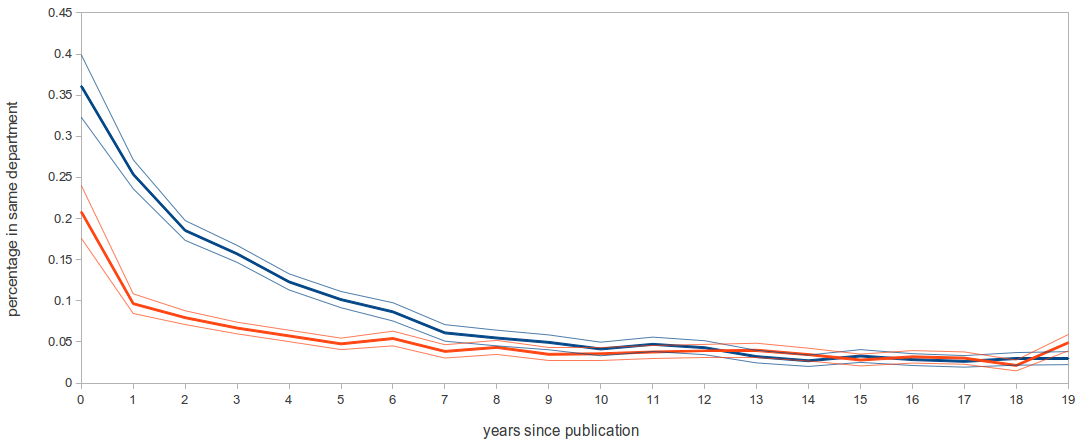
\includegraphics[scale=0.35]{pics/jaf_results_pooled.png}
\caption{Results of Jaffe exercise, Dark Blue = Citing Papers, Light Red =
Reference Papers}
\label{fig:jaf_ex}
\end{figure}

Citing papers are initially more likely to come from the same department
compared to reference papers, but the effect fades over time. A little
under a decade after a paper is published those outside the originating
department are just as likely as those in the department to cite the
originating paper. Like a disease, it takes knowledge of a paper some
time to diffuse outside the originating department. Similar results
using patent data were recorded in \citet{jaffe1993geographic}.

\subsection{Dealing with Endogenous Sorting}

The Jaffe exercise above recently came under attack.
\citet{thompson2005patent} redid the original exercise with more
detailed patent data, and nearly all of the important results in the
original were overturned. Applied to my situation, the Thompson critique
is that field does not adequately control for the endogenous sorting of
academics with similar interests into the same department. The reason I
observe departmental colleagues citing new research first may just be
that coworkers are the most interested in each other's work. Controlling
for field as I did in the Jaffe exercise above mitigates this problem,
but will not eliminate it completely. In Appendix \ref{sec:sortbias} a simple
related model shows that bias will make spillovers look stronger than they are.

In order to deal with possible bias, in a second exercise I control for
research interest more carefully and use an instrumental variable.
As in the structural exercise above, I will use the work of Michael Jensen.
I downloaded information on all the
citations of all of his papers, and collected the number of total times
each economist cited any of Jensen's papers as of 2013. An economist who
cites Jensen more often is more interested in Jensen's research. I then
choose a single Jensen paper, as above his 1986 \emph{American Economic Review} piece
``Agency costs of free cash flow, corporate finance, and takeovers''.

I record the year of first citation for each of the 669 academics who
ever cited the 1986 paper. My hypothesis is that, conditioning on interest in
Jensen's work, those who ever worked at Harvard will cite Jensen's paper
earlier. Let $CY_i$ be the year that author $i$ first cited the 1986 Jensen paper.
$Harv_i$ is a dummy which is set to 1 if author $i$ ever worked at Harvard. 
$Jcits_i$ is the total number of times author $i$ ever cited any of Jensen's 
papers.  I run the following regression:

\begin{equation}
    CY_i = \beta_0 + \beta_H Harv_i + \beta_J Jcits_i + \mathbf{\beta} \mathbf{X}_i + \varepsilon_i
    \label{eq:jens_love}
\end{equation}

Here $\mathbf{X}_i$ contains characteristics of author $i$ such as dummies for
the first year $i$ was observed in my data.  


\begin{table}[!ht]
    \begin{tabular}{lllll}
        \hline
                           & Citation year & Citation year & Citation year & Citation year \\ \hline \hline
        Worked at Harvard  & -2.38**       & -2.13*        & -2.04**       & -27.93**      \\
        Total Jensen cites & --            & -0.13***      & -0.10***      & -0.05         \\
        First year dummies & no            & no            & yes           & yes           \\
        Only first cohort  & no            & yes           & no            & no            \\
        Instrumented       & no            & no            & no            & yes           \\ \hline
        IV First Stage     &               &               &               & Worked at Harvard \\ \hline
        Quality            &               &               &               & .001***       \\
        Total Jensen cites &               &               &               & .002          \\
        First year dummies &               &               &               & yes           \\ \hline
        Obs                & 669           & 438           & 669           & 669           \\
        $R^2$              & 0.01          & 0.03          & 0.11          & --            \\ \hline 

    \end{tabular}
    \caption{Effect of working at Harvard on year of Jensen citation}
    \label{tab:jens_love}
\end{table}

Table \ref{tab:jens_love} contains the estimation results from \eqref{eq:jens_love}.
The only first cohort model uses only authors who were working in 1986.  The
correlations described in the table support the hypothesis that location matters.
In the simple OLS models of the first three columns, those who worked at
Harvard with Jensen cited him around two years earlier than others on
average, and for every other citation of Jensen's other work an author
cited Jensen's new paper on average a month or so earlier.

The instrument used in the last column is the quality of an academic measured by
mean coauthor-adjusted citations per published paper. The exogeneity
assumption is that quality is correlated with working at Harvard, but
quality only affects the timing of citing Jensen's paper through its
effect on location. The instrumented effect of working at Harvard is
both very strong and statistically significant. I ran placebo tests on
everything in the regression table using a Princeton, Berkeley, and
University of Pennsylvania dummy rather than a Harvard dummy. The
coefficients on the placebo dummies were never statistically
significant.

\clearpage
\section{Sorting and Bias}
\label{sec:sortbias}

Sorting of academics into departments is not random. People tend to work
alongside others with similar interests. The econometric challenge in
this paper is sorting out how working together affects citing behavior
and how having similar interests affects citing behavior. To motivate
the difficulty, suppose the hazard of citing a paper is observed, and
given by:

\begin{equation}
\lambda_{it} = \beta_0 + \beta_1 \mbox{dep\_frac}_{it} + \beta_2 \mbox{interest}_i + \varepsilon_{it}
\end{equation}

In words, the hazard of citing a paper depends on the fraction of
colleagues who know about the paper as well as personal interest in the
topic. Suppose that instead of estimating the true model above via OLS,
we estimated:

\begin{equation}
\lambda_{it} = \gamma_0 + \gamma_1 \mbox{dep\_frac}_{it} + \varepsilon_{it}
\end{equation}

It is a standard result that the asymptotic expected value for the
estimator $\hat{\gamma_1}$ can be written:

\begin{equation}
    \mathbb{E}[\hat{\gamma_1}] = \beta_1 + \rho_{\{\mbox{dep\_frac},\mbox{interest}\}} \sqrt{\frac{\sigma_{\mbox{interest}}^2}{\sigma_{\mbox{dep\_frac}}^2}}
\end{equation}

$\rho$ is the Pearson correlation coefficient, and here we expect it to
be positive. This specification, then, leads to an overestimation of the
effect of being in the same department on the hazard of citing a paper.
In most of this paper, I deal with similar bias by using a dummy for
working in the same field as a paper. Suppose that I now estimate the
following model:

\begin{equation}
    \lambda_{it} = \delta_0 + \delta_1 \mbox{dep\_frac}_{it} + \delta_2 \mbox{field} + \varepsilon_{it}
\end{equation}

Now we can write the asymptotic expected value of the estimator
$\hat{\delta_1}$ as (Hanushek and Jackson 1977):

\begin{equation}
    \mathbb{E}[\hat{\delta_1}] = \beta_1 + \frac{\rho_{\{\mbox{dep\_frac},\mbox{interest}\}} - \rho_{\{\mbox{dep\_frac},\mbox{field}\}}\rho_{\{\mbox{field},\mbox{interest}\}}}{1 - \rho_{\{\mbox{dep\_frac},\mbox{field}\}}^2} \sqrt{\frac{\sigma_{\mbox{interest}}^2}{\sigma_{\mbox{dep\_frac}}^2}}
\end{equation}

If field and interest are perfectly correlated, then the second term is
eliminated and the estimator is no longer biased. The less well field
acts as a proxy for interested, the more biased the estimator will be.
As long as we believe that field and interest are positively correlated,
the estimate of $\beta_1$ is biased upward.

Loosely speaking, this intuition goes through for all the exercises in
the paper. The second exercise in the reduced form section is an
exception. In that exercise I construct an interest variable more
detailed than field, and also use an instrument to help with
identification.

\clearpage
\section{Data Construction}
\label{sec:dat_cons}

\subsection{ISI Web of Knowledge}

My primary data source is the Thomson-Reuters Web of Knowledge
(http://thomsonreuters.com/web-of-knowledge/). The Web of Knowledge is a
citation database including conference proceedings, journal articles,
books, and patents. The Web of Knowledge is similar to other citation
databases such as Google Scholar. One difference is that Google Scholar
indexes working papers from a variety of sources, while the Web of
Knowledge tracks only published papers. For my purposes, the most
important distinction is that in the Web of Knowledge, there is a
uniform page for each paper containing summary details such as academic
names and affiliations. Google Scholar links to outside web pages which
each have different information formats.

Using the python library beautiful soup, I scraped data from the Web of
Knowledge. The program started with a list of all papers classified as
economics papers by the Web of Knowledge (a distinction based on the
journal the paper was published in), and clicked through the link to
each paper one at a time. Detailed information on the paper was then
recorded on my hard disk. In particular, I recorded the following
information for each paper:

\begin{enumerate}
\def\labelenumi{\arabic{enumi}.}
\itemsep1pt\parskip0pt\parsep0pt
\item
  Academic names
\item
  Academic affiliations
\item
  Paper Title
\item
  Journal Title
\item
  Number of citing papers
\end{enumerate}

In addition to getting this information for the most cited 100,000
economics papers, I also recorded the same information for every paper
(not necessarily economics) which either cited an economics paper
published in 1980, cited an economics paper published in 2005, or cited
one of the one hundred most cited economics papers of all time.

I cleaned and processed the data using a large data processing tool
called OpenRefine. I used the cleaned data to link academics to
departments. There were several difficulties in doing this. The first is
that I dropped all information about a department except the name of the
university. While university names are recorded fairly consistently in
the database, department information is not. One affiliation might list
Harvard University, Economics Dept. Another might list Harvard
University, Department of Economics, and still another might give no
department information at all. The upshot is that I conflate every
Harvard department together, so that the Harvard Business School, the
Kennedy School of Government, and the Economics Department are all
considered to be the same location for my purposes.

A second, similar problem is in recording the names of academics. First
and middle names are sometimes completely recorded, and sometimes only
initials are given. I dealt with this by dropping all first and middle
names except the first initial of the first name. This certainly causes
problems with common names, especially with Chinese names like Li. If
two Li's have the same first initials, they will be conflated in my
data.

Another difficulty is with academics who have several affiliations within
a given year. Many economists list the National Bureau of Economic
Research as a second affiliation, for instance. I dropped all NBER
affiliations, and dealt with other affiliation problems case by case.

\subsection{Constructing Fields}

\subsubsection{IDEAS Fields}

In the main structural exercise we need fields for each academic.
In some of the additional exercises reported in Section \ref{sec:add_evid}, we need
fields for papers as well. My main source for this information is IDEAS,
a database of economists hosted by the St.~Louis Federal Reserve Bank
(http://ideas.repec.org/). Ideas allows economists to register
themselves, report affiliation, and report current working papers and
publications. Using this information, IDEAS ranks economists and
institutions along a number of dimensions. Registering with IDEAS is
voluntary, and some 37,000 economists have registered.

IDEAS classifies economists into field based on something called the NEP
mailing lists. NEP, for New Economics Papers, curates new articles
appearing on ideas into 91 different categories. Each category is
curated by a particular economist, and over time people take turns being
curator. Every so often, in my experience about once a week, an email in
each category is sent out listing new papers. IDEAS puts academics into
categories based on which mailing list distributes their papers. If
either 5 of an economists papers have been included in a particular
mailing list, or at least 25\% of all of an economists papers have been
included, then the economist is deemed to be working in the field of the
mailing list.

The IDEAS website maintains a list of economists classified in this way
(http://ideas.repec.org/i/e.html). An economist can be classified as
working in any number of fields, at least any number of to 91. I again
used python and beautiful soup to record every economist affiliation on
IDEAS. This amounts to about 30,000 economists. In the structural
section, when I say that an economist has the same field as the Jensen
paper, I will mean that IDEAS lists him as working in either the field
of contract theory, or business economics.

\subsubsection{Journal Fields}

In some exercises in this study, a paper field is required as well. To
get a field for each paper, I combine the academic field described above
with a journal field. For the journal field, I use the classification of
\citet{barrett2000subdiscipline}. These classifications are JEL field,
which is different than the NEP field I have for academics. Using the JEL
classification descriptions from the JEL website, I linked the 91 NEP
fields to the JEL fields the journals were classified into. I first used
fuzzy matching on words in the field descriptions, and then went through
and hand corrected odd matches.

To construct the field for each paper, I added together the 91 x 1 field
vector of all of the academics, then added the 91 x 1 field vector of the
journal the paper was published in. I then normalized to that the
resulting vector is a unit vector. Distance between paper fields is then
the Euclidean distance between 91 x 1 field vectors.

\subsection{Simplifications}

As mentioned in the main body of the paper, I cut out all but the
top 104 departments when performing the structural estimation. Academics
at lower ranked departments publish more rarely, so that I do not
observe them very often making the affiliation data noisy. Table \ref{tab:dep_field} at
the end of this file is a sample of included departments and fields.

\begin{table}[!ht]
    \centering
    {\footnotesize
    \begin{tabular}{lll}
        \hline
        DEPT                     & QUAL  & JENS. FIELD \\ \hline \hline
        UNIV MICHIGAN            & 0.884 & 0.035       \\
        PURDUE UNIV              & 0.490 & 0.0036      \\
        PENN STATE UNIV          & 0.663 & 0.067       \\
        HARVARD UNIV             & 1.0   & 0.014       \\
        UNIV PENN                & 0.903 & 0.041       \\
        CORNELL UNIV             & 0.817 & 0.016       \\
        UNIV ROCHESTER           & 0.355 & 0.086       \\
        MIT                      & 0.980 & 0.086       \\
        UNIV MARYLAND            & 0.798 & 0.060       \\
        STANFORD UNIV            & 0.932 & 0.028       \\
        UNIV DELAWARE            & 0.346 & 0.0         \\
        CARNEGIE MELLON UNIV     & 0.625 & 0.047       \\
        YALE UNIV                & 0.923 & 0.026       \\
        PRINCETON UNIV           & 0.971 & 0.051       \\
        UNIV ILLINOIS            & 0.557 & 0.031       \\
        BOSTON UNIV              & 0.913 & 0.012       \\
        UNIV N CAROLINA          & 0.403 & 0.0         \\
        \ldots                   &       &             \\
        UNIV NEW MEXICO          & 0.038 & 0.140       \\
        CUNY HUNTER COLL         & 0.105 & 0.0         \\
        UNIV MIAMI               & 0.086 & 0.0         \\
        TUFTS UNIV               & 0.538 & 0.0         \\
        BRIGHAM YOUNG UNIV       & 0.336 & 0.0         \\
        UNIV CALIF IRVINE        & 0.644 & 0.0         \\
        UNIV HAWAII MANOA        & 0.144 & 0.0         \\
        EMORY UNIV               & 0.326 & 0.0         \\
        UNIV CALIF SAN DIEGO     & 0.855 & 0.056       \\
        WELLESLEY COLL           & 0.432 & 0.257       \\
        CUNY                     & 0.375 & 0.0         \\
        DREXEL UNIV              & 0.067 & 0.0         \\
        MIDDLEBURY COLL         & 0.182 & 0.0         \\
        SANTA CLARA UNIV         & 0.115 & 0.0         \\
        UNIV CALIF SANTA CRUZ    & 0.615 & 0.0         \\
        SUNY ALBANY              & 0.394 & 0.0         \\
        TULANE UNIV              & 0.317 & 0.192       \\
        APPALACHIAN STATE UNIV   & 0.269 & 0.0         \\
        RENSSELAER POLYTECH INST & 0.298 & 0.0         \\
        CHAPMAN UNIV             & 0.548 & 0.0         \\ \hline
    \end{tabular}}
    \caption{Selected departments.}
    \label{tab:dep_field}
\end{table}

\clearpage

\begin{table}[!ht]
    \centering
    {\footnotesize
    \begin{tabular}{ll}
        \hline
        NEP ABREV & FIELD NAME\\ \hline \hline
        NEP-ACC   & Accounting \& Auditing\\
        NEP-AFR   & Africa\\
        NEP-AGE   & Economics of Ageing\\
        NEP-AGR   & Agricultural Economics\\
        NEP-ARA   & Arab World\\
        NEP-BAN   & Banking\\
        NEP-BEC   & Business Economics\\
        NEP-CBA   & Central Banking\\
        NEP-CBE   & Cognitive \& Behavioural Economics\\
        NEP-CDM   & Collective Decision-Making\\
        NEP-CFN   & Corporate Finance\\
        NEP-CIS   & Confederation of Independent States\\
        NEP-CMP   & Computational Economics\\
        NEP-CNA   & China\\
        NEP-COM   & Industrial Competition\\
        NEP-CSE   & Economics of Strategic Management\\
        NEP-CTA   & Contract Theory \& Applications\\
                  &\\
        NEP-ORE   & Operations Research\\
        NEP-PBE   & Public Economics\\
        NEP-PKE   & Post Keynesian Economics\\
        NEP-POL   & Positive Political Economics\\
        NEP-PPM   & Project, Program \& Portfolio M\\
        NEP-PUB   & Public Finance\\
        NEP-REG   & Regulation\\
        NEP-RES   & Resource Economics\\
        NEP-RMG   & Risk Management\\
        NEP-SBM   & Small Business Management\\
        NEP-SEA   & South East Asia\\
        NEP-SOC   & Social Norms \& Social Capital\\
        NEP-SOG   & Sociology of Economics anagent\\
        NEP-SPO   & Sports \& Economics\\
        NEP-TID   & Technology \& Industrial Dynami\\
        NEP-TRA   & Transition Economics\\
        NEP-TRE   & Transport Economics\\
        NEP-TUR   & Tourism Economics\\
        NEP-UPT   & Utility Models \& Prospect Theo\\
        NEP-URE   & Urban \& Real Estate Economics \\ \hline

    \end{tabular}}
    \caption{Selected fields.}
\end{table}

\clearpage
\section{Verifying Contraction Mapping}
\label{sec:contr_map}

Let $T$ be the operator on the space of bounded functions $f$ on the
space $1,2,\dots,D$. In particular, let $T$ be defined as follows:

\begin{equation}
    (Tf)(d) = \rho \ln\left( \sum_{d' \in \mathcal{D}} e^{f(d') + w(d') - \mathbbm{1}_{\{d'\neq d\}} \ \mathcal{C}} \right)    
    \label{eq:operator}
\end{equation}

We will verify that $T$ is a contraction mapping using Blackwell's
sufficient conditions. Recall Theorem 3.3 from
\citet{stokey1989recursive}:

Theorem 3.3 (Blackwell's sufficient conditions for a contraction): Let
$X \subseteq \mathbb{R}^l$, and let $B(X)$ be a space of bounded
functions $f:X\rightarrow \mathbb{R}$, with the sup norm. Let
$T: B(X) \rightarrow B(X)$ be an operator satisfying:

\begin{enumerate}
\def\labelenumi{\alph{enumi}.}
\itemsep1pt\parskip0pt\parsep0pt
\item
  (monotonicity) $f, g \in B(X)$, and $f(x) \leq g(x)$, for all
  $x \in X$, implies $(Tf)(x) \leq (Tg)(x)$, for all $x$ in $X$.
\item
  (discounting) there exists some $\beta \in (0,1)$ such that
  $[T(f + a)](x) \leq (Tf)(x) + \beta a$, for all $f \in B(X) $,
  $a \geq 0$, $x\in X$.
\end{enumerate}

In \eqref{eq:operator}, monotonicity is immediate.  Discounting is almost
immediate as well. Take $a \geq 0$, and let $f(x) \in B(X)$:

\begin{align}
    [T(f + a)](d) &= \rho \ln \left( \sum_{d'} \left(e^{f(d') + w(d') - \mathbbm{1}_{\{d'\neq d\}}\mathcal{C} + a}\right)\right) \nonumber \\
    &= \rho \ln \left( e^a \sum_{d'} \left(e^{f(d') + w(d') - \mathbbm{1}_{\{d'\neq d\}}\mathcal{C}}\right)\right) \nonumber \\
    &= (Tf)(d) + \rho a \nonumber \\
\end{align}

Both monotonicity and discounting hold, so by Blackwell's sufficient conditions the operator $T$ is a contraction.

\clearpage
\section{Deriving Emax Expectation}
\label{sec:exp_der}

In this appendix, I show that if $X$ and $Y$ are constants, and $\varepsilon_1$ and $\varepsilon_2$ are distributed IID Gumbel (0,1), then:\footnote{My Russian officemates tell me that this is just trivial probability theory.  Even so, I saw the result in several papers which all referenced \citet{rust1987optimal}, but it is not derived there either!  I leave the derivation here for future puzzled American graduate students.}

\begin{equation}
    \mathbb{E} \left[\max\{X + \varepsilon_1, Y + \varepsilon_2\}\right] = \gamma_e + \ln \left(e^{X} + e^{Y}\right)
    \label{eq:rust_eq}
\end{equation}

The CDF of the Gumbel distribution is $F(z) = e^{-e^{-z}}$, so we can write the distribution of the maximum in \eqref{eq:rust_eq} as:

\begin{equation}
    G(z) = e^{-\left(e^{X - z} + e^{Y - z}\right)}
\end{equation}

Take the derivative with respect to $z$ to get the PDF:

\begin{equation}
    g(z) = \left(e^{X - z} + e^{Y - z}\right) e^{-\left(e^{X - z} + e^{Y - z}\right)}
\end{equation}

Now we can rewrite the LHS of \eqref{eq:rust_eq} as:

\begin{equation}
    \int_{-\infty}^\infty z g(z) dz 
\end{equation}

Use the change of variable $t = e^{X - z} + e^{Y - z}$ (the trick is that $\ln(t) = \ln\left(e^X + e^Y\right) - z$):

\begin{equation}
    \int_{0}^\infty \left(\ln \left(e^X + e^Y\right) - \ln(t)\right) e^{-t} dt = \ln \left(e^X + e^Y\right) + \gamma_e
\end{equation}

The substitution of $\gamma_e$ is an identity.\footnote{This identity can be found in both the Wikipedia and Wolfram Mathworld articles on the Euler-Mascheroni constant.  The Wolfram article references the textbook \citet{whittaker1996course} after a list of identities involving $\gamma_e$, but I was not able to find this particular identity there.}

\clearpage
\section{MCMC Diagnostics}
\label{sec:MCMC_diag}

\begin{figure}[!ht]
    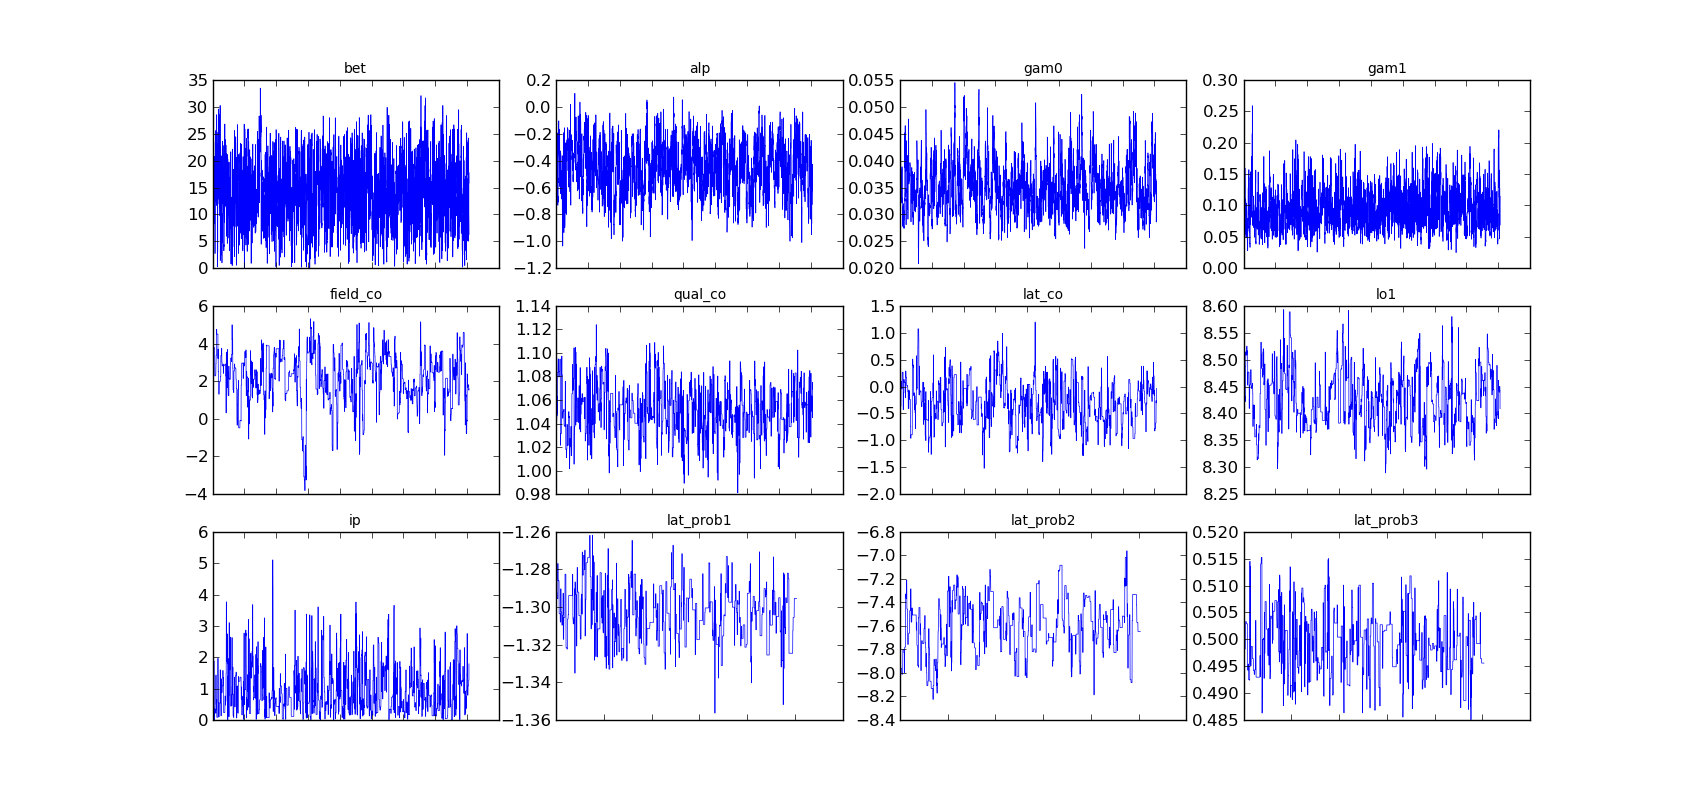
\includegraphics[scale=0.35]{pics/params_plots_big.png}
    \caption{Mixing plots}
    \label{fig:mix}
\end{figure}

This appendix presents mixing plots and diagnostics from the parallel
MCMC estimation. Eyeballing the plots in Figure \ref{fig:mix}, everything looks good.  Eyeballing,
however, is not very reliable.
Table \ref{tab:grtest} presents Gelman-Rubin convergence criterion results. Recall that to pass the
Gelman-Rubin convergence criterion, the test value must be below 1.1.
All parameters pass the Gelman-Rubin test.

\begin{table}[!ht]
    \centering
    \begin{tabular}{lll}
        \hline
        parameter       & GR criterion \\ \hline \hline
        $\alpha$        & 1.013  \\
        $\beta$         & 1.003  \\
        $\gamma_{F}$    & 1.019  \\
        $\gamma_{NF}$   & 1.005  \\
        $\xi_f$         & 1.016  \\
        $\xi_l$         & 1.008  \\
        $\xi_q$         & 1.029  \\
        $\phi_Q$        & 1.070  \\
        $\phi_F$        & 1.034  \\
        $\sigma$        & 1.073  \\
        $\mathcal{C}$   & 1.010  \\
        $\xi_{ex}$      & 1.013  \\ \hline
    \end{tabular}
    \caption{Gelman-Rubin Test}
    \label{tab:grtest}
\end{table}

\clearpage
\section{Patent vs Academic Citations}

Citations are footprints left behind by ideas moving between brains. If
an academic uses an old idea in a new paper, he cites it. At least since
the late 1980's, researchers have used citation data to measure the
spread of ideas, although more often the citations have been of patents
rather than academic citations \citep{griliches1998patent}. Some
researchers have been explicit about why they prefer patent data.
\citep{jaffe2002patents} write: ``Academics may cite a friend (or
neighbor) just to be nice, since the price of doing so is infinitesimal,
or even negative if a longer list of references is perceived as making
the research look more thorough. An inventor who did the same is in
effect leaving money lying on the table: if those citations are included
in the final patent, the inventor has reduced the scope of her
monopoly.'' Few understand the language of \emph{quid pro quo} better
than academics, but the problem of undeserved citation is no less severe
in patenting. It isn't clear to me how citing an irrelevant patent hurts
an inventor. In fact, the value of a patent is related to the number of
other patents which cite it, so there is an incentive for inciting there
as well.

In some ways academic citations are better than patent citations at
measuring knowledge diffusion. The rules for who is listed as inventor
on a patent are as complicated as a rocket schematic. In a 1972 legal
opinion, Judge Newcomer of the Eastern Pennsylvania Circuit Court
reflected on the meaning of
inventorship:\footnote{352 F. Supp. 1357; 1972 U.S. Dist. LEXIS 10602; 176 U.S.P.Q. (BNA) 361. LexisNexis Academic. Web. Date Accessed: 2013/07/30.}

\begin{quote}
{[}Joint inventorship{]} is one of the muddiest concepts in the muddy
metaphysics of the patent law. On the one hand, it is reasonably clear
that a person who has merely followed instructions of another in
performing experiments is not a co-inventor\ldots{}To claim
inventorship\ldots perhaps one need not be able to point to a specific
component as one's sole idea, but one must be able to say that without
his contribution to the final conception, it would have been less --
less efficient, less simple, less economical, less something of benefit.
\end{quote}

Due to difficulties with inventorship, the patent literature has been
confined to studying the flow of ideas between firms. Since academic
citations follow clear norms for authorship, I can use my data to
understand how ideas spread within firms as well. The bar for authorship
does differ between academic fields. In economics coauthors can usually
be counted on one (invisible) hand, while it is not unusual for papers
published in Nature to have more than 100 authors
\citep{greene2007demise}.

A second advantage of using academic citation data is seeing the dogs
that did not bark. My panel includes academics who did not cite a paper,
often departments full of non-citers. In this respect academic citation
data is even richer than most epidemiology data. The epidemiologists
from whom I derive my model work with data on only households with at
least one influenza infection. If I were using patent citation data, I
would not have information on the pool of people who might have cited a
patent. Information on non-citers will make my estimates more precise.

\clearpage
\section{Discussion of Long-Run Behavior of Movement Model}
\label{sec:movdists}

In this section I simulate the long-run distribution of academics over departments
in the baseline structural model, and compare to the empirical
distribution in the data.  Using the 1994 distribution of academics over departments
as the initial distribution, I simulated the model for 1000 years.  The first 500
years were thrown out as a burn-in.

\begin{figure}[!ht]
    \centering
    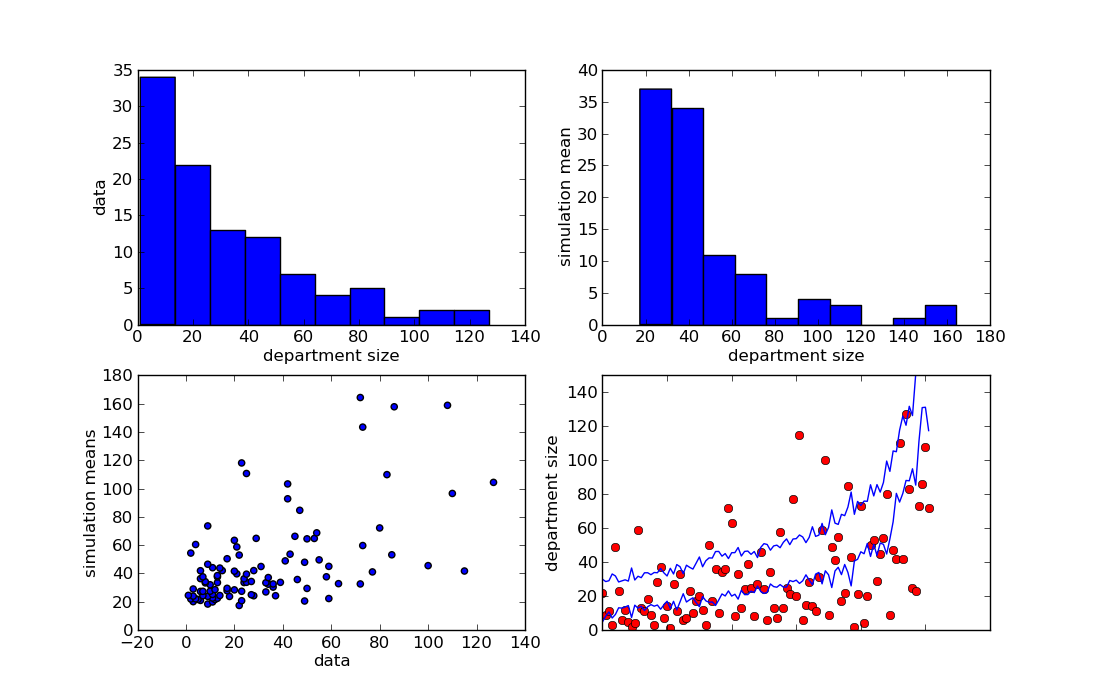
\includegraphics[scale=0.5]{pics/mov_plts.png}
    \caption{TL: Histogram of data, TR: Histogram of simulation means, BL: Scatter plot data vs. simulation means, BR: Two standard deviations of simulation variation against data.}
    \label{fig:mov_plts}
\end{figure}

The top row of Figure \ref{fig:mov_plts} contains a histogram of the data department sizes
and a histogram of simulated mean department sizes.  The histograms are qualitatively similar,
although there are no very small departments in the simulation.  The scatter plot in the 
lower-left panel compares department sizes in the data to simulated mean department sizes.
While there is positive relationship between the data and the simulation
means, the correlation is far from perfect. The Pearson correlation coefficient is 0.39.

Even in the long-run, department sizes fluctuate as opportunities to move stochastically
arise.  The bottom right panel of Figure \ref{fig:mov_plts} plots bounds
of two standard deviations around the simulated mean department size (the two lines), as well
as the 1994 data (the dots).  Departments are ordered on the x-axis according to size of
simulated mean department size.  The simulation cannot account for 
the smallest department sizes observed in the data.  It is not unexpected that the long-run department sizes
implied for the model differ somewhat from the
department size distribution observed in 1994.  The model
developed above has nothing to say about entry or exit, and during this period the economics
profession is growing rapidly.

\clearpage
\section{Robustness Check: Estimating with an Alternative Paper}
\label{sec:gross}

In this appendix I present a table comparing the baseline Jensen estimates to a re-estimation using
\citet{grossman1986costs}.  This is a slightly older version of the model in the baseline section.  As can be seen in Table \ref{tab:post_comp}, the estimates are almost 
identical.

\begin{table}[!ht]
    \centering
    \begin{tabular}{lllll}
        \hline
         & \multicolumn{2}{c}{Baseline}        & \multicolumn{2}{c}{Grossman Hart} \\ \hline\hline
                            & mean    & std   & mean       & std    \\ 
         $\alpha$           & -0.651  & 0.163 & -0.456     & 0.176  \\ 
         $\beta$            & 19.272  & 6.402 & 17.394     & 6.069  \\ 
         $\gamma_{F}$       & 0.089   & 0.028 & 0.089      & 0.004  \\ 
         $\gamma_{NF}$      & 0.034   & 0.004 & 0.034      & 0.029  \\ 
         $\xi_f$            & 0.973   & 0.910 & 1.100      & 0.881  \\ 
         $\xi_l$            & 0.666   & 0.182 & 0.675      & 0.174  \\ 
         $\xi_q$            & 0.404   & 0.031 & 0.403      & 0.032  \\ 
         $\lambda_o$        & 0.045   & 0.002 & 0.045      & 0.002  \\ 
         $\phi_F$           & -21.586 & 0.282 & -21.575    & 0.281  \\ 
         $\sigma$           & 0.820   & 0.009 & 0.820      & 0.008  \\ 
         $\xi_{ex}$         & 0.266   & 1.276 & 0.225      & 0.827  \\ \hline
    \end{tabular}
    \caption{Posterior moment comparison}
    \label{tab:post_comp}
\end{table}

\clearpage
\section{Posterior Kernal Densities for Alternative Models}
\label{sec:altmodels}

\begin{figure}[!ht]
    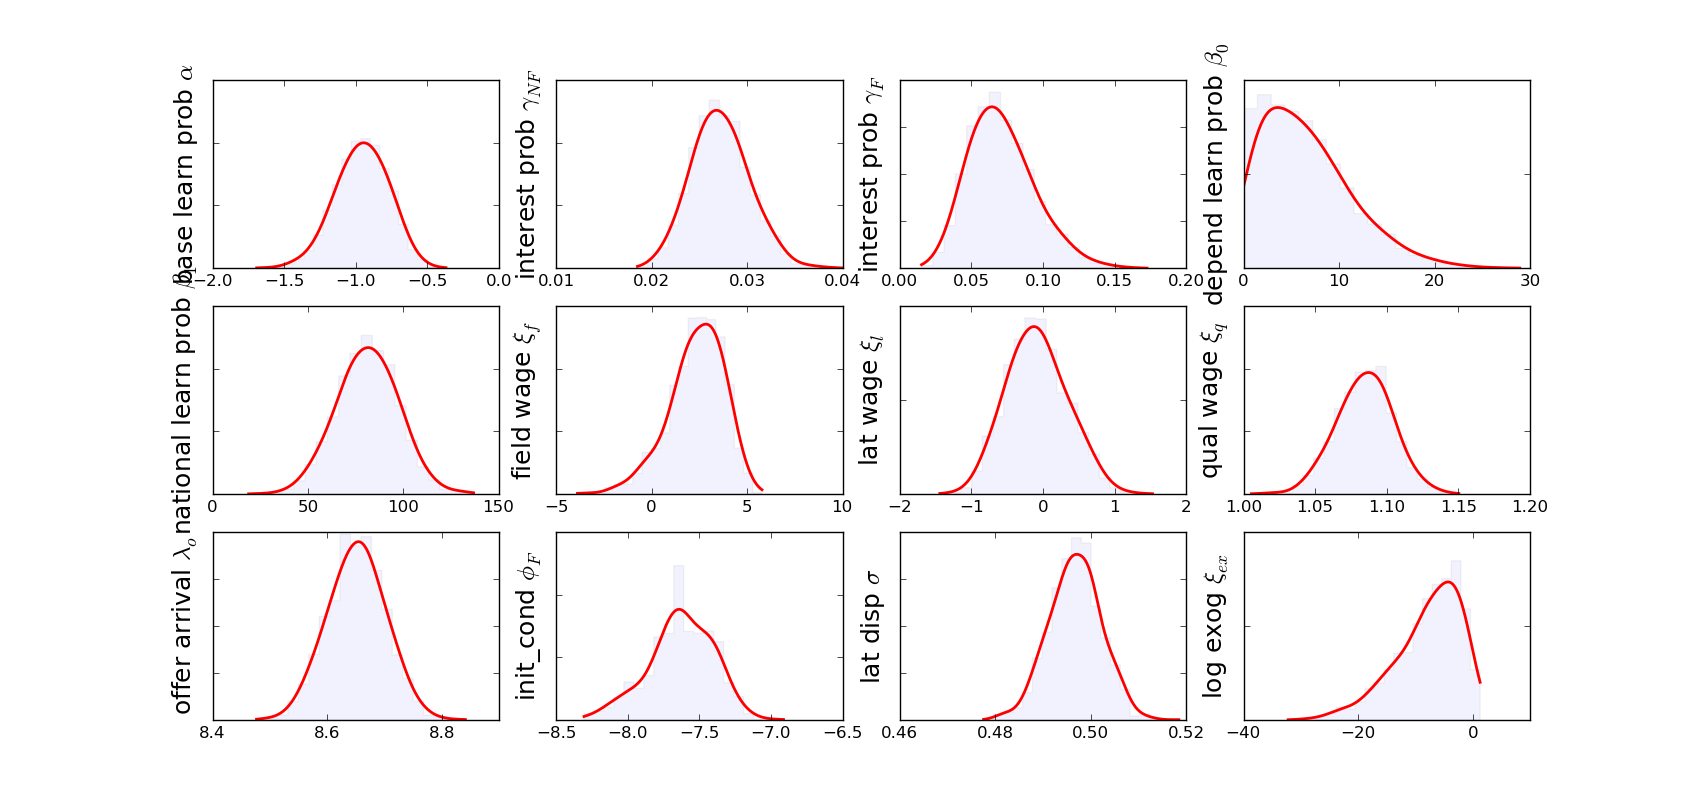
\includegraphics[scale=0.35]{pics/params_dists_reg.png}
    \caption{Posteriors for national model}
\end{figure}

\begin{figure}[!ht]
    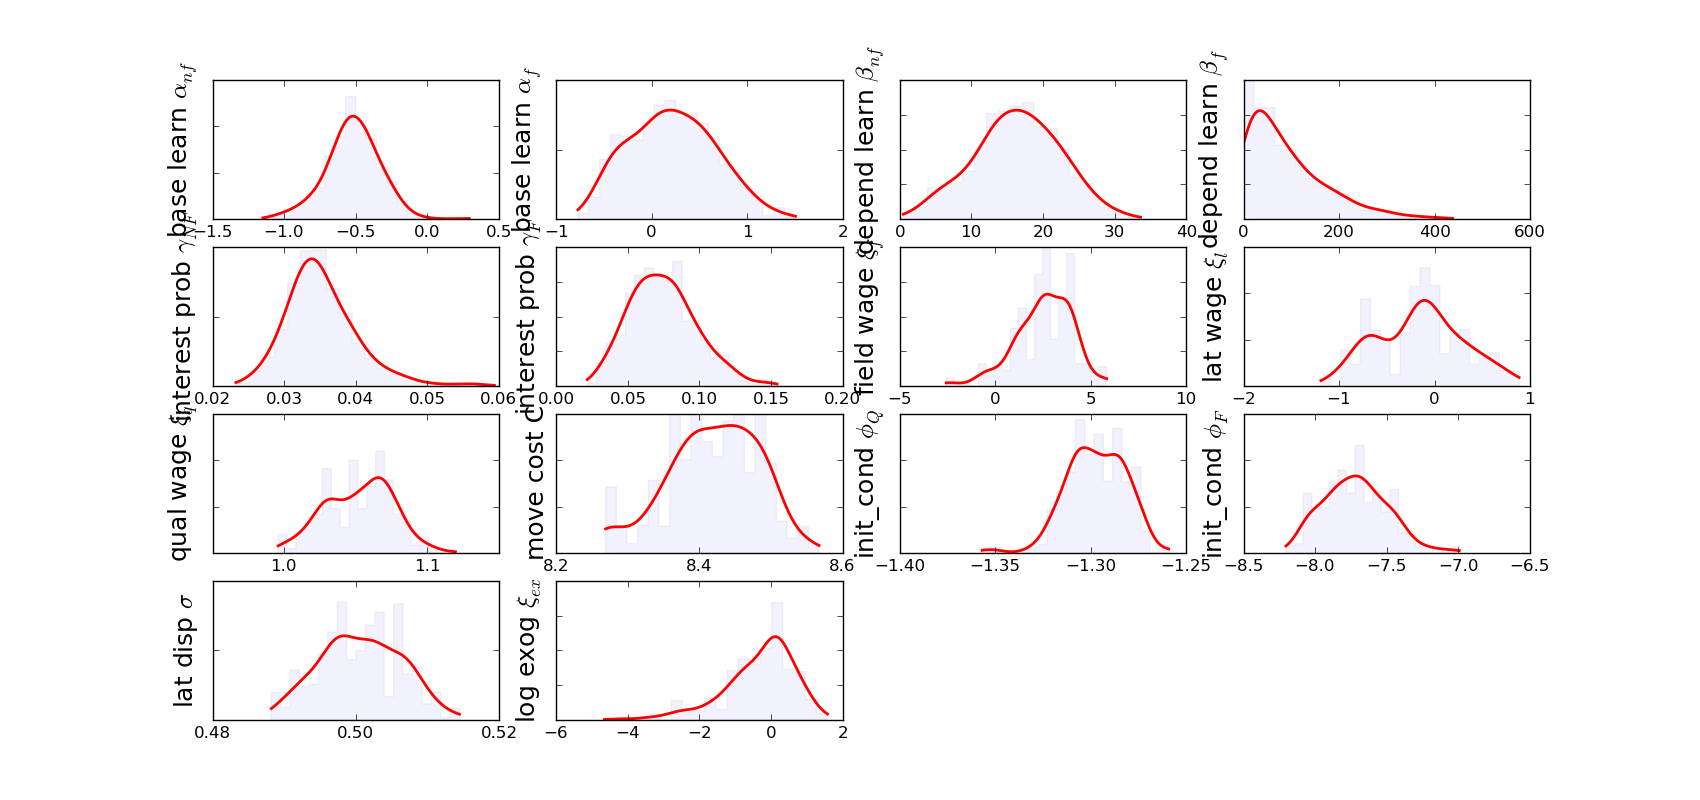
\includegraphics[scale=0.35]{pics/params_dists_split.png}
    \caption{Posteriors for field-specific model}
\end{figure}

\begin{figure}[!ht]
    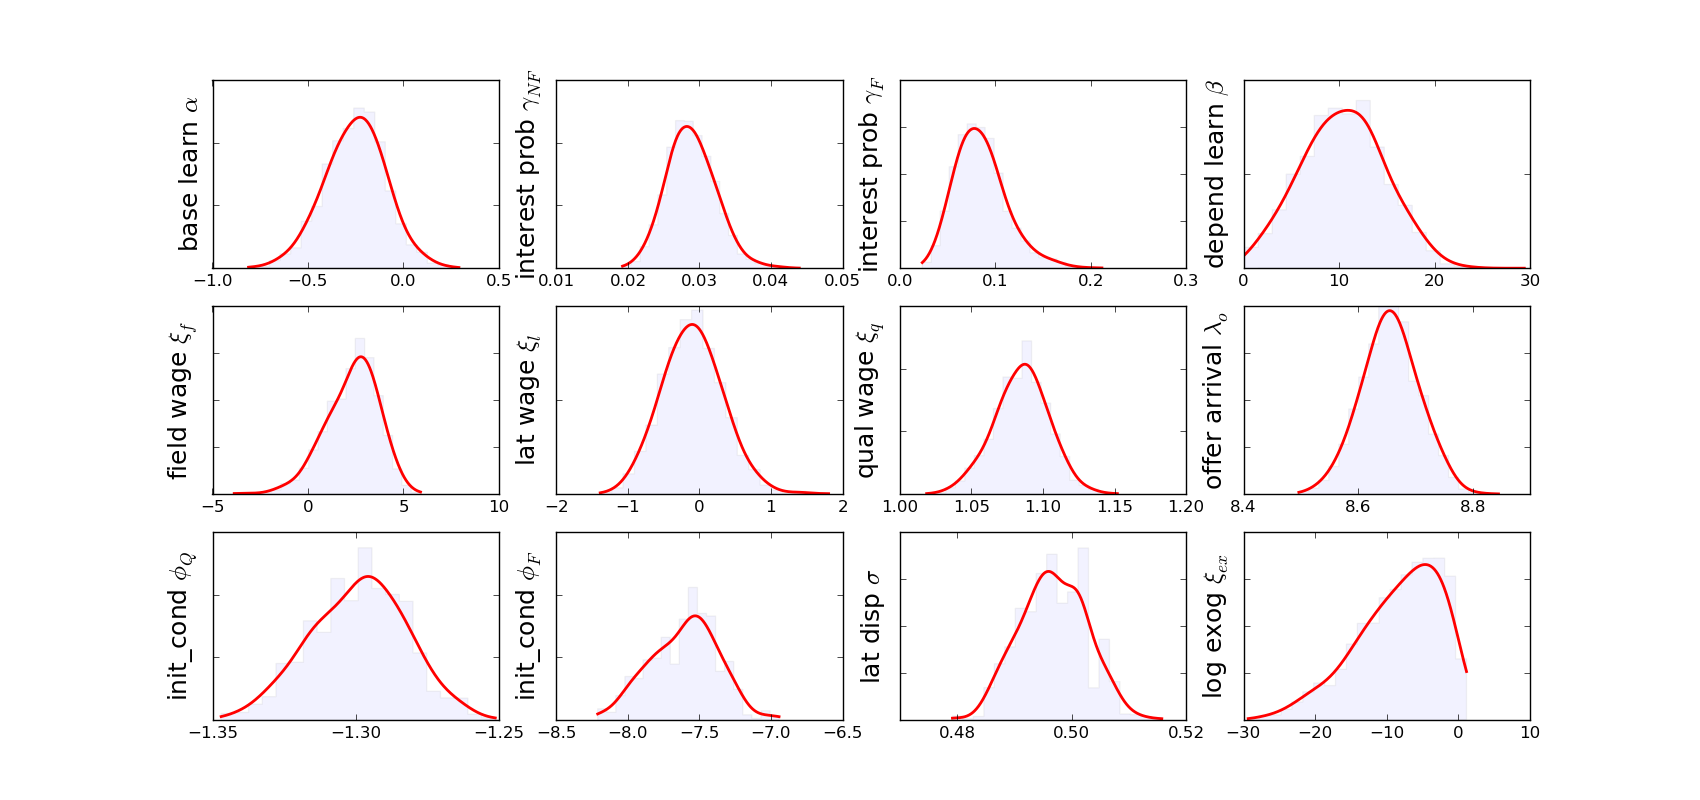
\includegraphics[scale=0.35]{pics/params_dists_lag.png}
    \caption{Posteriors for publication lag model}
\end{figure}

\clearpage 

\section{Comparison of Baseline Priors} 
\label{sec:prior_comp}

\begin{table}[!ht]
    \centering
    \begin{tabular}{lllll}
        \hline
         & \multicolumn{2}{c}{Exponential (300)}        & \multicolumn{2}{c}{Diffuse} \\ \hline                            & mean    & std   & mean       & std    \\ \hline \hline
         $\alpha$             & -0.447 & 0.179 & -0.628 & 0.178 \\ 
         $\beta$              & 14.128 & 5.850 & 15.992 & 6.466 \\ 
         $\gamma_{F}$         & 0.035  & 0.004 & 0.034  & 0.004 \\ 
         $\gamma_{NF}$        & 0.094  & 0.031 & 0.091  & 0.030 \\ 
         $\xi_f$              & 2.208  & 1.374 & 2.246  & 1.557 \\ 
         $\xi_l$              & -0.293 & 0.411 & -0.061 & 0.428 \\ 
         $\xi_q$              & 1.050  & 0.021 & 1.084  & 0.019 \\ 
         $\mathcal{C}$        & 8.426  & 0.052 & 8.655  & 0.052 \\ 
         $\phi_Q$             & -1.302 & 0.014 & -1.300 & 0.015 \\ 
         $\phi_F$             & -7.603 & 0.230 & -7.588 & 0.227 \\ 
         $\sigma$             & 0.499  & 0.005 & 0.496  & 0.005 \\ 
         $\xi_{ex}$           & 0.919  & 0.739 & 0.021  & 0.126 \\ \hline 
    \end{tabular}                              
    \caption{Posterior moment comparison, alternate priors}
    \label{tab:prior_comp}
\end{table}
